%\section{Impossibility of SNOW properties with two clients with restricted communication }\label{two-client}
\section{Two Client Open Question}
\label{sec:2c2s}
This section closes the open question of whether SNOW properties can be implemented with two clients. We first prove that SNOW remains impossible in a 2-client 2-server system if the clients cannot directly send messages to each other.
% We prove our result by showing 
 %a contradiction. 
 However, in the presence of client to client communication, it is possible to have all SNOW properties with two clients and at least two servers.
 %Fig~\ref{fig:architecture2a}.
 
 \subsection{No  SNOW Without C2C  Messages}
 \label{subsec:no_snow_no_c2c}
 
 
 In this section, we prove the following results that states it is impossible guarantee the SNOW properties in a transaction processing system with two clients, without client-to-client communication.
  \begin{theorem}\label{thm:two-snow}
  	The SNOW properties cannot be implemented in a system with two clients and two servers, where the clients do not communicate with each other.
  \end{theorem} 
 
 We use the same system model as in Section~\ref{sec:formal_proof}: two servers $s_x$ and $s_y$ with two clients, a reader $r_1$ that issues only 
\rots{} and a writer $w$ that issues only \wots{}. A \wot{} $W$ writes $(x_1, y_1)$ to $s_x$ and $s_y$, and a \rot{} $R$ reads both servers. We assume that there is a bi-directional communication channel between any pair of client and server and any pair of servers. There is no communication channel between clients. We assume that each transaction can be identified by a unique number, e.g., transaction identifier. 

%We denote the automata for servers $s_x$ and $s_y$ by $s_x$ and $s_y$, respectively, and the automata for the clients  $r$ and $w$ by $r$ and $w$, respectively.   
 %We denote by $S_1$  the subsystem consisting of $s_x$, $s_y$ and $w$,  and  by $S_1$  the  automata composed of  $s_x$, $s_y$ and $w$, i.e., $s_x \times s_y \times w$. 
 %Also, we  denote by $\mathcal{A}$, which can also be interpreted as the algorithm, the automaton representing the entire system consisting of $S_1$ and $r$ (i.e., $s_x \times  s_y$ $ \times w$ $ \times r$).  
% We assume that between any client $c$, 
 %$c \in \{r, w \}$ and any server $s$,  $s \in \{s_x, s_y\}$ there are  channel automata $Channel_{c, s}$ and $Channel_{s, c}$.
%Again, with abuse of notation we denote by $\mathcal{S}$ the automata composed of the automatons $s_x$, $s_y$ and $w$. Also, by $\mathcal{T}$ we denote the composition of automaton $\mathcal{S}$ and $r$, i.e., represents the entire system.  
%We used the notation $\writeop{o}{v}$ to mean a write operation with value $v$ on object $o$; and similarly, by $\readop{o}$ we mean a read operation on $o$.
%We  denote by $S_2$ the system, and also the  composed automaton,  consisting of  $s_x$, $s_y$, $r$ and  $w$, by composing the automatons $S_1$ and $r$, i.e., the automaton $S_1 \times r$.
%We assume that clients are non-faulty.
%Here, we consider only   executions of some algorithm ${\mathcal A}$ that satisfied SNOW properties.
%For contradiction, we  also assume that  any execution of $\mathcal{A}$  respects  the SNOW properties. 
% Also, we assume that in an execution $\epsilon$ of $\mathcal{A}$  we can identify each transaction with a unique identifier.

%\sloppy Consider an execution of ${\mathcal A}$ with  two transactions in it as:   a \wot{}  $W \equiv $ $WRITE($$ (o_1, x_1),  (o_2, y_1) )$ invoked by  $w$, where $x_1 \neq x_0$ and $y_1 \neq y_0$; and a \rot{}   $R \equiv READ$$(o_1, o_2)$, invoked by $r_1$.  
%Let us denote by 
%$op_x^{r_1}$ and $op_y^{r_1}$  the read operations $\readop{o_1}$ and  $ \readop{o_2} $, respectively.
%Due to the wait-free requirement for  the \wots{}, $W$ completes, and we denote by $\INV{W}$ the invocation action and $\RESP{W}$ the response action in $\alpha$. 
%
%\paragraph{Notations and Definitions:}
%We  introduce  the following notations and definitions in the context of an execution $\epsilon$, of $\mathcal{A}$, with transactions $R_1$ and $W$ in it.
%
%\begin{notation}
%We introduce the following notations for   actions relevant to $R$ in $\epsilon$,
% where  $ j \in \{1, 2\}$:
%\begin{enumerate}
%\item $\INV{R}$ and  $\RESP{R}$:  invocation and  response actions for  $R$,  at  $r$; 
%\item $\INV{W}$ and   $\RESP{W}$: invocation and  response actions for  $W$, at $w$;

%\item $\send{m_j^{r}}{r, s_j}$: an  output action at $r$,  which sends a message $m_j^{r}$ from reader $r$ to server $s_j$, requesting the value for $o_j$;
%\item $\recv{m_j^{r}}{r, s_j}$: an input action at $s_j$, that receives the message $m_j^{r}$, sent from $r$;
%\item $\send{v_j}{ s_j, r}$: an output action at $s_j$,  that  sends value $v_j$, for   $o_j$, to $r$.
%\item $\recv{v_j}{ s_j, r}$: an input action at $r$,  to receive a message $v_j$ from $s_j$ at  $r$.
%
%\end{notation}
%
%\begin{definition}
%\item  \emph{Non-blocking fragments $\frag{i}{\epsilon}$, $i \in \{1, 2\}$.}
 %Suppose there is a fragment of  execution  in $\epsilon$  where the first action is   $recv(m_i^r)_{r, s_i}$ and  the last action is 
 %$send(v_i)_{s_i, r}$ , both of which  occur  at $s_i$. Moreover, suppose there is  
% no other input action at $s_i$ in this fragment. Then we call this execution fragment 
  % a \emph{non-blocking response fragment} for $op_i^r$ at  $s_i$.  We use the notation  $\frag{i}{\epsilon}$ to denote this fragment of 
  %execution of $\epsilon$. %Similarly, if such an execution fragment occurs  with $m_y^r$, $y$ and $s_y$ then we denote this by  $\frag{1,y}{\epsilon}$ and refer to it as a non-blocking response fragment for $op_2^r$ at  $s_y$.
 %\end{definition} 


%\begin{notation}
 %\item  We use the notations $R(\epsilon)$ and $W(\epsilon)$ to denote the transactions $R$ and $W$, in $\epsilon$. When the underlying execution is clear from the context we simply use $R$ and $W$.
%\end{notation}

%\begin{notation}
% \item If the non-blocking fragment $\frag{1,x}{\epsilon}$ appears in $\epsilon$ such that $recv(m^{r_1}_2)_{r, s_y}$, at $s_y$,  does not occur before
% $\frag{1,x}{\epsilon}$ completes and $\epsilon$ is of the form 
% $\finiteprefix{\ell-1}{\ell} \circ \frag{1,x}{\epsilon} \circ \frage{S}{\epsilon}{}$, where 
%$\frage{S}{\epsilon}{}$ is any continuation of the execution, then we denote $\finiteprefix{\ell-1}{\ell} $ by $\prefix{\epsilon}$.
 
%\item \sloppy If $\epsilon$ is of the form  
% $\finiteprefix{\ell-1}{\ell}  \circ \frag{1,x}{\epsilon} \circ \kappa \circ \frag{1,y}{\epsilon} , a_p, \sigma_p, \ldots$  or 
% $\finiteprefix{\ell-1}{\ell}  \circ \frag{1,y}{\epsilon} \circ \kappa \circ \frag{1,x}{\epsilon} \circ \frage{S}{\epsilon}{}$, where  
% $\ell$ is a positive integer, 
% $\kappa$ is a segment of $\epsilon$,  possibly even of length zero and $\frage{S}{\epsilon}{}$ is any suffix part of the execution 
% then we denote $\finiteprefix{\ell-1}{\ell} $ by $\prefix{\epsilon}$. Clearly,  we can write $\epsilon$ as $\prefix{\epsilon} \circ \frag{1,x}{\epsilon}\circ \kappa \circ \frag{1,y}{\epsilon} \circ \suffix{\epsilon}$ or $\prefix{\epsilon} \circ \frag{1,y}{\epsilon}\circ \kappa \circ \frag{1,x}{\epsilon} \circ \suffix{\epsilon}$.
%\end{notation}
%\end{enumerate}

 %However, unlike in the case of \rots{}, for \wots{} the SNOW properties do not impose strict conditions on the occurrence of external events at the clients or the servers. 
%However,  the  W property guarantees termination of any \wot{}. Therefore, all we can claim is  $\RESP{W}$ eventually appears after  $\INV{W}$.


Our strategy is still proof by contradiction: We assume there exists some algorithm $\mathcal{A}$ that satisfies all SNOW properties, and then we show the existence of a sequence of executions of $\mathcal{A}$, eventually leading to an execution that contradicts  the S property.
 %If $\epsilon$ is an execution of $\mathcal{A}$, with \rot{} $R$.
%  We denote by  $\frag{1,x}{\epsilon}$ and $\frag{1,y}{\epsilon}$  the execution fragments of $\epsilon$  between  the actions $recv(x)_{ s_x, r}$ and  $send(m_x^r)_{r, s_x}$ at $s_x$; and   $recv(x)_{ s_x, r}$ and  $send(m_y^r)_{r, s_y}$ at $s_y$, respectively, and in  $\frag{1,x}{\epsilon}$ and $\frag{1,y}{\epsilon}$  no other internal actions occur at $s_x$ and $s_y$, respectively.
 First,  we show the existence of an execution $\alpha$ of $\mathcal{A}$ where 
$R_1$ is invoked after $W$ completes, where the  send actions $send(m_x^{r_1})_{r_1, s_x}$ and $send(m_y^{r_1})_{r_1, s_y}$  at the  $r_1$  occur consecutively 
in  $P(\alpha)$, which is a prefix of $\alpha$. 
 Then we show that $\alpha$  can be written in the form  
$\prefix{\alpha} \circ \frag{1,x}{\alpha}$ (Fig.~\ref{fig:execution1} $(a)$, Lemma~\ref{lem:exec_alpha}). 
%\delete{where  the receive and response occurs at $s_x$ without any input action at $s_x$ between these two actions (Fig.~\ref{fig:execution1} $(a)$). }
 We then prove the existence of  another  execution $\beta$, which can be written in the form $\prefix{\beta} \circ \frag{1,x}{\beta} \circ \frag{1,y}{\beta}$ by extending $\alpha$ with an execution fragment $\frag{1,y}{\beta}$, such that $\frag{1,x}{\beta} \stackrel{s_x}{\sim} \frag{1,x}{\alpha}$
  (Fig.~\ref{fig:execution1} $(b)$; Lemma~\ref{lem:exec_beta}).
Note that in  any arbitrary extension of $\beta$, $R_1$ eventually returns $(x_1, y_1)$.
  %
Next, we show the existence of an execution $\gamma$ of the form  $\prefix{\gamma} \circ \frag{1,x}{\gamma} \circ \frag{1,y}{\gamma}$,  
 where the send actions $send(m_x^{r_1})_{r_1, s_x}$ and $send(m_y^{r_1})_{r_1, s_y}$  at  $r_1$ occur before $W$ is invoked (Fig.~\ref{fig:execution1} $(c)$; $\gamma$), but 
$\frag{1,x}{\gamma}$  and $\frag{1,y}{\gamma}$
occur after $\RESP{W}$ as in $\beta$.
%
%
Based on $\gamma$, we show the existence of an execution $\delta$ 
of the form  $\prefix{\eta} \circ \frag{1,x}{\eta} \circ \frag{1,y}{\eta}\circ \suffix{\eta}$, where 
  $R_1$ responds with $(x_1, y_1)$.
%
 %of $\mathcal{A}$ such that, $R$ is invoked before $W$ is invoked and $R$ completes after $W$.
 % Additionally, in $\beta$ the servers
  %$s_x$ and $s_y$ receive the object value requests from $r$ after $W$ completes and $R$ responds with $(x_1, y_1)$
   %From $\gamma$, we show the existence of an execution  $\eta$ of $\mathcal{A}$ where $F_1$ occurs before $F_2$,   and eventually  $R$ responds with $(x_1, y_1)$. 
   %
    Finally, starting with  $\eta$, we create a sequence of executions $\delta (\equiv \eta)$, $\delta^{(1)}$, $\cdots$ $\delta^{(f)}$, of $\mathcal{A}$, 
     where in each of them $R_1$ responds with $(x_1, y_1)$  (Fig.~\ref{fig:execution2} $(e)$ and $(g)$; Lemma~\ref{thm:two-snow}). Additionally,  for any $\delta^{(i)}$, the fragments   $\frag{1,x}{\delta^{(i)}}$ and
    $\frag{1,y}{\delta^{(i)}}$  appear before $\delta^{(i-1)}$.
    % i.e., $\prefix{\delta^{(i)}}$ is a prefix of $\prefix{\delta^{(i-1)}}$. 
    Based on $\delta^{(f)}$, we prove the existence of an execution $\phi$ (Fig.~\ref{fig:execution2} $(h)$), where $R_1$ returns 
    $(x_1, y_1)$ even before $W$ begins, which violates the $S$ property.

  
  Now, we explain the relevant lemmas used by the main proof. Due to space constraints, we present their proof in Appendix~\ref{app:2c-no-c2c}. The first lemma states that there exists a finite execution of ${\mathcal A}$, where $R_1$ begins after  
  $W$ completes, and the actions $send(m_x^{r_1})_{r_1, s_x}$ and $send(m_y^{r_1})_{r_1, s_y}$  occur 
before either of the servers $s_x$ and  $s_y$ 
  receives $m_x^{r_1}$ or $m_y^{r_1}$ from $r_1$;  also,  server $s_x$ responds to $r_1$ in a non-blocking manner (execution $\alpha$ in Fig.~\ref{fig:execution1}).  
\begin{lemma}\label{lem:exec_alpha} 
There exists a finite execution $\alpha$ of $\mathcal{A}$ that contains transactions $R_1(\alpha)$  
 and $W(\alpha)$ where $\INV{R}$ appears after $\RESP{W}$, and the following conditions hold:
\begin{enumerate}
\item[$(i)$] The actions $send(m_x^{r_1})_{r_1, s_x}$ and  $send(m_y^{r_1})_{r_1, s_y}$ appear consecutively in $trace(\alpha)|r_1$; and 
\item[$(ii)$]   $\alpha$ contains the execution fragment  $\frag{1,x}{\alpha}$.
%, i.e., the actions  $recv(m_x^r)_{r, s_x}$ and  $send(x)_{r, s_x}$ appear in $trace(\alpha)|s_x$, where  there is no input action of  $s_x$  between these actions.
% \item[$(ii)$]  $R(\alpha)$ returns  $(x_1, y_1)$. 
\end{enumerate} 
\end{lemma}

\remove{
\begin{proof}
Consider a finite  execution fragment  of $\mathcal{A}$ with a completed transaction $W$, where  after $W$ 
completes  the adversary invokes $R$, i.e., $\INV{R_1}$ occurs.
 Note that each of the  read operations $op_1^{r_1}$ and $op_2^{r_1}$,  in $R_1$,  can be invoked by the adversary at any point in the execution.  
 Following $\INV{R}$,  the adversary introduces the invocation action $\inv{op_1^r}$;  by the O property of the read operations of $\mathcal{A}$  
the action $send(m_x^{r_1})_{r_1, s_x}$ eventually occurs. Next, the adversary introduces 
 $\inv{op_2^{r_1}}$ and also, delays the arrival of  $m_x^{r_1}$ until  action $send(m_y^{r_1})_{r_1, s_y}$ eventually occurs, 
 which  must occur in accordance with  the property O  of read operations. Let us call this finite execution $\alpha^0$. 
 
 Next, suppose at the end of $\alpha^0$  the adversary delivers the message $m_x^{r_1}$, which has been delayed so far, 
 via the action  $recv(m_x^{r_1})_{r, s_x}$, 
 at  $s_x$,   but  it delays any  other input actions at $s_x$. Note that by the $N$ property of read operations $s_x$ eventually responds with  $send(x)_{s_x, r_1}$, with one value $x$ by o property,  where $x = x_1$ by the S property, since $R$ begins after $W$ completes. 
 Let us call this execution $\alpha$. Note that $\alpha$ satisfies conditions $(i)$ and $(ii)$ by the design of the execution.
\end{proof}
}

% The following lemma states that starting from execution $\beta$ we show that there exists an execution of ${\mathcal A}$ such that $R$ initiates after $W$ completes  such that,  the send events from the reader occur first (see execution $\beta$ in Fig.~\ref{fig:execution1} $(b)$).  
 %
 %{If $\alpha$ is an execution of $\mathcal{A}$, with \rot{} $R$. We denote by  $\frag{1,x}{\alpha}$ and $\frag{1,y}{\alpha}$  the execution fragments of $\alpha$  between  $recv(x)_{ s_x, r}$ and  $send(m_x^r)_{r, s_x}$ at $s_x$; and   $recv(x)_{ s_x, r}$ and  $send(m_y^r)_{r, s_y}$ at $s_y$, respectively. During  $\frag{1,x}{\alpha}$ and $\frag{1,y}{\alpha}$ no other internal actions occur at $s_x$ and $s_y$, respectively.}

   The following lemma states that there is an execution $\beta$ where $R$ begins after  $W$ completes, and the two send events at $r_1$ occurs before  $\frag{1,x}{\beta}$, which thus occurs before $\frag{1,y}{\beta}$ ($\beta$ in Fig.~\ref{fig:execution1}).  
   
  
\begin{lemma}\label{lem:exec_beta} 
There exists an  execution $\beta$ of $\mathcal{A}$ that contains transactions $R_1$ and $W$ where $\INV{R_1}$ appears after $\RESP{W}$ and the following conditions hold:
\begin{enumerate}
\item[$(i)$] The actions $send(m_x^{r_1})_{r_1, s_x}$ and  $send(m_y^{r_1})_{r_1, s_y}$ appear consecutively in $trace(\beta)|r_1$; and
\item[$(ii)$]   $\beta$ contains the execution fragment  $\frag{1,x}{\beta} \circ \frag{1,y}{\beta}$.
% $recv(m_x^r)_{r, s_x}$,  $send(x)_{r, s_x}$,  $recv(m_y^r)_{r, s_y}$,  $send(y)_{r, s_y}$, where  there is no external action, in $\beta$,  of  $s_x$ and $s_y$ between these actions.
% \item[$(iii)$] $R(\beta)$ returns $(x_1, y_1)$. 
\end{enumerate} 
\end{lemma}
\remove{
\begin{proof}
Consider the  execution $\alpha$ of $\mathcal{A}$ as constructed in Lemma~\ref{lem:exec_alpha}.  
At the end of the execution fragment $\alpha$,  the adversary  delivers the previously delayed message
 $m_y^r$, which is sent via the action $send(m_y^r)_{r, s_y}$,  by  introducing the action $recv(m_y^r)_{r, s_y}$. The adversary then delays any other  input action in $\mathcal{A}$. By the N property,  
server $s_y$ must respond to $r$, with some value $y$,  and hence 
the output action $send(y)_{s_y, r}$ must eventually occur at $s_y$.  
Let us call this finite execution as $\beta$. Note that $\beta$ satisfies the  properties $(i)$ and $(ii)$ in the statement of the lemma.
\end{proof}
}


 The following result shows  that starting with $\beta$  there is an execution 
 $\gamma$, where  $R_1$ is invoked before $W$ is invoked while
  $send(m_x^{r_1})_{r_1, s_x}$ and  $send(m_y^{r_1})_{r_1, s_y}$  occur before $\INV{W}$ (Fig.~\ref{fig:execution1} $(c)$) and $m_x^{r_1}$ and $m_y^{r_1}$ from $r_1$ reach $s_x$ and $s_y$ after the action  $\RESP{W}$.  


\begin{lemma}\label{lem:exec_gamma} 
There exists an execution $\gamma$ that contains $R_1$ and $W$, where the action $\INV{R_1}$ appears before $\INV{W}$ and $\RESP{R_1}$ appears after  $\RESP{W}$, and the following conditions hold for $\gamma$:
\begin{enumerate}
\item[$(i)$] The actions $send(m_x^{r_1})_{r_1, s_x}$ and  $send(m_y^{r_1})_{r_1, s_y}$  appear before $\INV{W}$ and they appear consecutively in $trace(\gamma)|r_1$;
%\item[$(ii)$]   $trace(\beta)$ contains the sequence  $recv(m_x^r)_{r, s_x}$,  $send(x)_{r, s_x}$,  $recv(m_y^r)_{r, s_y}$,  $send(y)_{r, s_y}$.
\item[$(ii)$]   $\gamma$ contains the execution fragment  $\frag{1,x}{\gamma} \circ \frag{1,y}{\gamma}$; and 
\item[$(iii)$] action $\RESP{W}$ occurs before $\frag{1,x}{\gamma}$.
\end{enumerate} 
\end{lemma}

\remove{
\begin{proof}
Consider the execution $\beta$ of $\mathcal{A}$  as in Lemma~\ref{lem:exec_beta}. Note that $\beta$
is an execution of the composed automaton $\mathcal{A}$ ($\equiv S_1 \times r$).  In $\beta$,  the actions 
 $send(m_x^r)_{r, s_x}$ and   $send(m_y^r)_{r, s_y}$ occur at $r$; and following that,  the actions 
 $recv(m_x^r)_{r, s_x}$, $recv(m_y^r)_{r, s_y}$, $send(x)_{s_x, r}$ and  $send(y)_{s_y, r}$ occur at $S_1$. 
 Consider the executions $\alpha_r \equiv \beta|r$ and  $\alpha_{S_1} \equiv \beta|S_1$. Let $s_{\beta}$ denote  $trace(\beta)$.
 
 In $s_{\beta}$, $send(m_x^r)_{r, s_x}$,  $send(m_y^r)_{r, s_y}$ appear after $\RESP{W}$, as in $trace(\beta)$. Let $s'_{\beta}$ be the sequence of
 external actions of $S_2$ which we construct from $s_{\beta}$ by moving $send(m_x^r)_{r, s_x}$,  $send(m_y^r)_{r, s_y}$ before $\INV{W}$, which  is also 
 an external action of $\mathcal{A}$, and leaving the rest of the actions in $s_{\beta}$ as it is.
 
 
 In $\beta$,  $\INV{R}$, $recv(x)_{ s_x, r}$ and  $recv(y)_{s_y, r}$ 
  are the only input actions at $r$, therefore,   $s'_{\beta} |r= trace(\alpha_r)$. 
  %
  On the other hand,  $recv(m_x^r)_{r, s_x}$, $recv(m_y^r)_{r, s_y}$ are the only input actions at $s_x$ ,
   therefore, $s'_{\beta} |S_1 = trace(\alpha_{S_1})$.  Now, by Theorem ~\ref{thm:paste}, there exists an execution 
 $\gamma$ of $\mathcal{A}$ such that, $s'_{\beta} = trace(\gamma)$ 
 and $\alpha_r = \gamma|r$ and $\alpha_{S_1} = \gamma|S_1$. Therefore, 
 in $\gamma$, $send(m_x^r)_{r, s_x}$,  $send(m_y^r)_{r, s_y}$ appear before
  $\INV{W}$ (condition $(i)$) and since $s'_{\beta} = trace(\gamma)$ condition $(ii)$  holds. Conditions $(iii)$ holds trivially.
\end{proof}
}

\remove{
In the following lemma we show  that in any   execution, of ${\mathcal A}$,  that is  an extension of either execution $\beta$ or execution  $\gamma$, as in  the preceding lemmas, $R_1$ eventually returns $(x_1, y_1)$.

\begin{lemma}\label{lem:exec_xi}
Let $\xi$  be an execution of $\mathcal{A}$ that is an   extension of the either  execution $\beta$ from Lemma~\ref{lem:exec_beta} or execution  $\gamma$ from Lemma~\ref{lem:exec_gamma},  then  $R(\xi)$  responds with $(x_1, y_1)$.
\end{lemma}

\begin{proof}
Note that in executions $\beta$ and $\gamma$,  the traces $trace(\beta)|s_x$  is a prefix of $trace(\gamma)|s_x$, since  $\beta$ ends with
$\frag{1,x}{\beta}$ and $\gamma$ ends with $\frag{1,y}{\gamma}$
Therefore, in both $\beta$ and $\gamma$, the  respective $send(x)_{s_x, r}$ actions have the same value for their  $x$'s. 
Now, in  any extended  execution $\eta$ of $\mathcal{A}$, which starts 
with $\beta$ or $\gamma$, by the properties $N$ and $O$ the transaction $R$ completes;  and  by the property $S$,   $R$ returns  $(x_1, y_1)$.
Therefore,  $R_1(\xi)$  returns $(x_1, y_1)$.
\end{proof}
}

 In the following lemma, we show there exists an    execution $\eta$  of  
$\mathcal{A}$  of the form 
$\prefix{\eta}\circ \frag{1,x}{\eta} \circ \frag{1,y}{\eta} \circ \suffix{\eta}$
where  $\RESP{R}$ appears in  $\suffix{\eta}$  (Fig.~\ref{fig:execution1} $(d)$) and 
$R(\eta)$ returns $(x_1, y_1)$. 

\begin{lemma}\label{lem:exec_delta} 
There exists an execution $\eta$ of $\mathcal{A}$ that contains transactions $R$ and $W$ where $\INV{R}$ appears before $\INV{W}$;  $\RESP{R_1}$ appears after  $\RESP{W}$ and the following conditions hold for $\eta$:
\begin{enumerate}
\item[ $(i)$] $\eta$ can be written in the form $\prefix{\eta}\circ \frag{1,x}{\eta} \circ \frag{1,y}{\eta} \circ \suffix{\eta}$, for some 
   $\prefix{\eta}$ and $\suffix{\eta}$;
\item[$(ii)$] The actions $send(m_x^r)_{r_1, s_x}$ and  $send(m_y^{r_1})_{r_1, s_y}$  
appear before  $\INV{W}$ and they appear consecutively in $trace(\eta)|r_1$;
\item[$(iii)$] action $\RESP{W}$ occurs before $\frag{1,x}{\eta}$; and 
 \item[$(iv)$] $R_1(\eta)$ returns $(x_1, y_1)$. 
\end{enumerate} 
\end{lemma}

\remove{
\begin{proof}
Let $\gamma$ be an execution of $\mathcal{A}$, as described in Lemma~\ref{lem:exec_gamma}. 
%Without loss of generality, suppose   $recv(m_x^r)_{r, s_x}$ occurs in $\gamma$ before  $recv(m_y^r)_{r, s_y}$. 
 Let $\gamma^0$ be the execution fragment of $\gamma$
up to the action $send(y)_{s_y, r}$. Now, by Theorem~\ref{thm:extension} (1), there exists an execution $\gamma^0 \circ \mu$, of 
$\mathcal{A}$, where $\mu$ denotes the extended portion of the execution.

% with the empty sequence for $\beta$, in the theorem statement.  Now, due to the N and O properties of an execution of $\mathcal{A}$ the
%action $send(x)_{r, s_x}$ occurs in $\gamma^0 \circ \mu$ (in $\mu$, to be precise).
%Let $\mu^0$ be the prefix of $\mu$ with its last output action as  $send(x)_{r, s_x}$. Again, using Theorem~\ref{thm:extension} (3), with $\beta$ consisting of only $recv(m_y^r)_{r, s_y}$, we create an execution of $\mathcal{A}$ that starts with $\gamma^0 \circ \mu^0$.
 Clearly, by the N and O properties, 
%executions of $\mathcal{A}$ 
the actions  $\resp{op_1^r}$ and $\resp{op_2^r}$ must eventually occur in $\gamma^0 \circ \mu$.
%We can write $\nu$ as $\nu^0\circ \eta^0$ such that it ends with the action  $send(y)_{r, s_y}$.
 Now,  identify $\eta$ as $\gamma^0 \circ \mu$,  where $\prefix{\eta} \circ \frag{1,x}{\eta} \circ \frag{1,y}{\eta}$  is $\gamma^0$,   and $\mu$ is $\suffix{\eta}$, thereby, proving condition $(i)$.

Note the condition $(ii)$ is satisfied by $\eta$ because $\RESP{W}$ appears in $\prefix{\eta}$, therefore, the execution $\gamma$ is equivalent to the execution fragment of $\prefix{\eta}$ up to the event $\INV{W}$, and  also, 
$\gamma$ satisfies condition $(ii)$ as stated in Lemma~\ref{lem:exec_gamma}.

Condition $(iii)$ is true because $\frag{1,x}{\eta}$ begins with action $recv(m_x^r)_{r, s_x}$, which occurs after $\RESP{W}$.
Condition $(iv)$ is satisfied by $\eta$ because $\eta$ is an extension of $\gamma$ and due to  the result of Lemma~\ref{lem:exec_xi}.
\end{proof}
}

  %Next we define another execution fragment $\gamma$, of  $S_2$, as follows. Consider the execution fragment $\prefix{\alpha}{ \RESP{W}}$, i.e.,  up to the point in $\alpha$ when $W$ completes. Now we create an execution fragment $t$ of $S_2$, such that 
  %$t|S_2 = \prefix{\alpha}{ \RESP{W}}$ and does not contain any output action of  $R$. Next we create execution fragment  $\gamma$ from $t$, by  adding action $\INV{R}$ at $r$ to $t$,  before $\INV{T_w}$,as in the case of $\beta$.

\remove{
  \begin{figure}[!ht]
      \centering
         %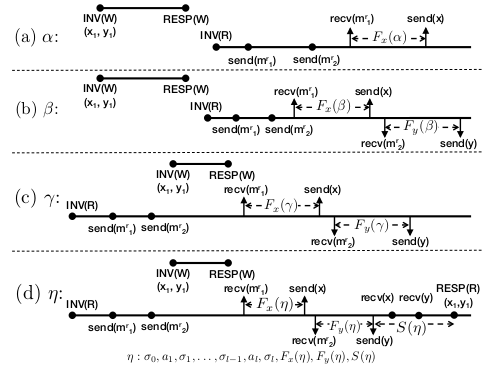
\includegraphics[scale=0.60]{figures/fig4.pdf} 
         %KMK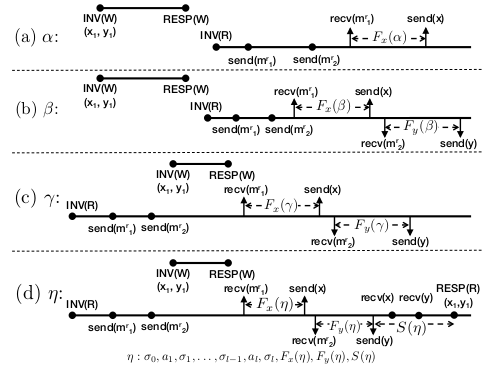
\includegraphics[width=4in]{figures/fig4.png} 
         \vspace{-2.0em}
         \caption{
\small{Schematic representation of executions $\alpha$, $\beta$, $\gamma$ and $\eta$,
          of ${\mathcal A}$ with transactions $R$ and $W$. The executions evolve from left to right. 
          The dots denote external events at clients. 
          The up-arrow marks denote external actions at $s_x$. The down-arrow marks denote external actions at $s_y$.}} \label{fig:execution1}
 \end{figure}

\begin{figure}[!ht]
      \centering
         %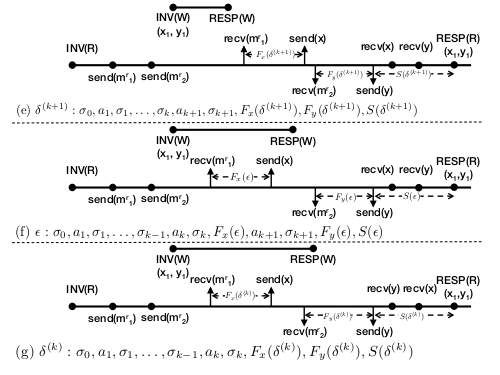
\includegraphics[width=1.00\textwidth]{figures/fig5.pdf} 
         %KMK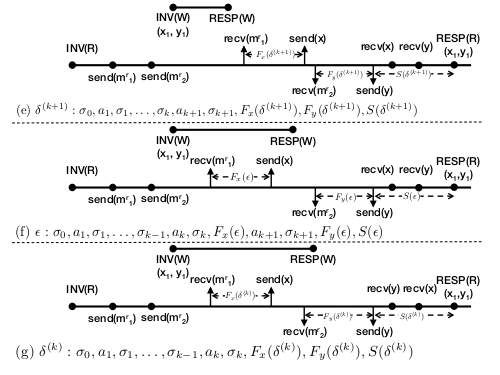
\includegraphics[width=4in]{figures/fig5.png}
         \vspace{-2.0em}
        \caption{\small{Executions $\delta^{(k+1)}$, $\epsilon$, and $\delta^{(k)}$, which show a progressive sequence of executions that are built on execution $\eta$ in Fig.~\ref{fig:execution1}.}}
         %\caption{\small{From execution $\eta$ of $\mathcal{A}$,  the construction of the progressive sequence of executions 
         %$\delta, \delta', \ldots$,  of  $\mathcal{A}$, of the form $\prefix{\cdot } \circ \frag{1,x}{\cdot}\circ \frag{1,y}{\cdot} \circ \suffix{\cdot}$. 
%The final execution $\phi$ of $\mathcal{A}$ to contradict the S property.}} 
      \label{fig:execution2}
\vspace{-1em}
 \end{figure}
}


\begin{figure}[t]
	%\centering
	\hspace*{-1.3cm}
	\begin{subfigure}{0.49\columnwidth}
		\centering
	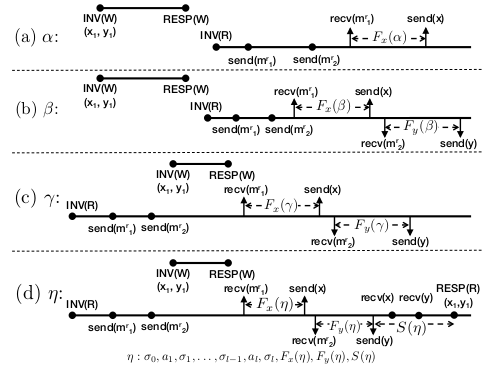
\includegraphics[width=1.2\linewidth]{figures/fig4.png}
	\end{subfigure}
	\hspace*{0.7cm}  
	\begin{subfigure}{0.49\columnwidth}
		\centering
	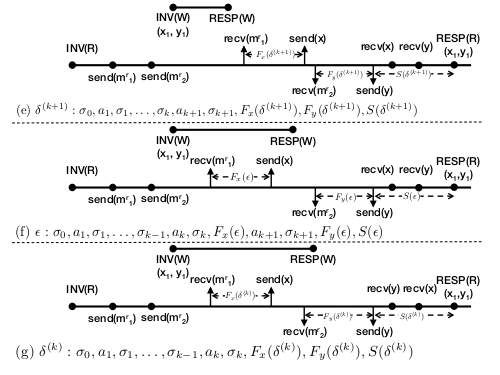
\includegraphics[width=1.2\linewidth]{figures/fig5.png}
	\end{subfigure} 
	         \caption{
	         	\small{Schematic representation of executions $\alpha$, $\beta$, $\gamma$ and $\eta$,
	         		of ${\mathcal A}$ with transactions $R$ and $W$. The executions evolve from left to right. 
	         		The dots denote external events at clients. 
	         		The up-arrow marks denote external actions at $s_x$. The down-arrow marks denote external actions at $s_y$.}} \label{fig:execution1}
\end{figure}



\remove{
\begin{figure}[t]
\centering
\begin{subfigure}{1.0\columnwidth}
\centering
  \includegraphics[width=1.0\linewidth]{figures/fig4-1.pdf}
\end{subfigure}  
\begin{subfigure}{1.0\columnwidth}
\centering
  \includegraphics[width=1.0\linewidth]{figures/fig4-2.pdf}
\end{subfigure}  
\begin{subfigure}{1.0\columnwidth}
\centering
  \includegraphics[width=1.0\linewidth]{figures/fig4-3.pdf}
\end{subfigure}  


\caption{\small{try graphs}}
%% High level performance comparison between \eigermoon and Eiger with latency-throughput graph and comparisons on system overall throughput with varying degrees of skewness and write fractions.
%% Throughput comparison when varying system load and latency comparison of read-only transactions. Data staleness is measured by comparing \eigermoon to a linearizable baseline.}
\label{fig:latency}
\end{figure}
}


  The following proof proves Theorem~\ref{thm:two-snow}. In the proof we start with an execution $\eta$ and create a sequence of executions of 
  $\mathcal{A}$, where each one is of the form $\prefix{\cdot} \circ \frag{1,x}{\cdot}\circ \frag{1,y}{\cdot}\circ \suffix{\cdot}$, with progressively shorter $\prefix{\cdot}$ until we have a final execution that contradicts the $S$ property.
\remove{
 \begin{theorem}\label{thm:two-snow}
 The SNOW properties cannot be implemented in a system with two clients and two servers, where the clients do not communicate with each other.
\end{theorem}
}

\begin{proof}
\sloppy Consider an execution $\delta^{(\ell)}$  of $\mathcal{A}$ as in Lemma~\ref{lem:exec_delta}, and let $\prefix{\delta^{(\ell)}}$  be the execution fragment
$\finiteprefix{\ell-1}{\ell}$.
%, where $\ell$ is some positive integer, and $\sigma_i$'s and $a_i$'s denote states and actions, respectively. 
By  Lemma~\ref{lem:exec_delta}, $\RESP{R_1(\delta^{(\ell)})}$  returns
 $(x_1, y_1)$ and $\delta^{(\ell)}$ is also of the form    
$\finiteprefix{\ell-1}{\ell} \circ \frag{1,x}{\delta^{(\ell)}} \circ \frag{1,y}{\delta^{(\ell)}} \circ \suffix{\delta^{(\ell)}}$.     
%Below we will show that from $\delta$ we can create another execution $\delta^{(\ell-1)}$ of the form $\finiteprefix{\ell-2}{\ell-1} \circ \frag{1,x}{\delta^{(\ell-1)}} \circ \frag{1,y}{\delta^{(\ell-1)}} \circ \suffix{\delta^{(\ell-1)}}$ where   $\RESP{R(\delta^{(\ell-1)})}$  returns $(x_1, y_1)$. Note that $\prefix{\delta^{(\ell-1)}}$ ($\equiv  \finiteprefix{\ell-2}{\ell-1} $) is a prefix of $\prefix{\delta^{(\ell)}}$.

Next, we inductively prove the existence of a finite sequence of executions of $\mathcal{A}$---i.e., by proving the existence of a new execution based on the existence of a previous one---as $\delta^{(\ell)}, \delta^{(\ell-1)}, \cdots \delta^{(i)}, \delta^{(i-1)},  \cdots \delta^{(f)}$, 
for some positive integer $f$, with the following properties: $(a)$ Each of the execution in 
the sequence can be written in the form  $\finiteprefix{i-1}{i} \circ \frag{1,x}{\delta^{(i)}} \circ \frag{1,y}{\delta^{(i)}} \circ \suffix{\delta^{(i)}}$ (or $\prefix{\cdot}\circ \frag{1,x}{\cdot}\circ \frag{1,y}{\cdot}\circ\suffix{\cdot}$); $(b)$ for each $i$, $f \leq i  < \ell$, we have  $\prefix{\delta^{(i)}}$ to be a prefix of $\prefix{\delta^{(i+1)}}$; and $(c)$ $R_1(\delta^{(f)})$  returns  $(x_0, y_0)$, and for any $i$,  $f <  i \leq \ell$,  we have   $R_1(\delta^{(i)})$  that returns  $(x_1, y_1)$.  Note that there is a final execution of the form $\delta^{(f)}$  because of the initial values of $x_0$ and $y_0$  and the \wot{}  $W$. 

%and $(d)$  the $\frag{1,x}{\delta^{(f)}}\circ \frag{1,y}{\delta^{(f)}}$   occurs before $\INV{W}$ in $\delta^{(f)}$. 

%The claims $(a)$, $(b)$ and $(c)$ is due to Lemma~\ref{two:induction}, and $(d)$ follows from the fact that $\prefix{\delta^{(\ell)}}$ is a finite prefix.

%\end{proof}
 
%\begin{proof}
 %Consider  $\delta$ which is of the form 
%$\finiteprefix{k}{k +1} \circ \frag{1,x}{\delta} \circ \frag{1,y}{\delta} \circ \suffix{\delta}$, where   transaction 
%$R(\delta)$ responds with 
%$(x_1, y_1)$.
Clearly, there exists an integer $k$,  $ f \leq  k < \ell$, such that $\frage{R}{\delta^{(k)}}{}$ returns $(x_0, y_0)$ and $\frage{R_1}{\delta^{(k+1)}}{}$ returns $(x_1, y_1)$. Now we start with execution 
$\delta^{(k+1)}$ and construct an execution $\delta^{(k)}$ as described in the rest of the proof. The following argument will show that  $\frage{R}{\delta^{(k)}}{}$ must also return $(x_1, y_1)$, which contradicts the assumption of having the $S$ property.

Consider the execution $\delta^{(k+1)}$ of the form 
$\finiteprefix{k}{k +1} \circ \frag{1,x}{\delta^{(k+1)}} \circ \frag{1,y}{\delta^{(k+1)}} \circ \suffix{\delta^{(k+1)}}$. 
 The action  $a_{k+1}$ can  occur at any of the automata $r$, $w$, $s_x$, and $s_y$. Therefore, we consider the following four possible cases.
%

\emph{ \underline{Case (i) $a_{k+1}$ occurs at $w$:}} The execution fragments
 $\frag{1,x}{\delta^{(k+1)}}$ and $\frag{1,y}{\delta^{(k+1)}}$ do not contain any input action  at $s_x$ or $s_y$. $a_{k+1}$ does not occur at $s_x$ or $s_y$. 
 %Therefore, the action $a_{k+1}$ cannot have any impact on them. 
 Therefore,
 the asynchronous network can
  delay the occurrence of $a_{k+1}$ at $w$ to create the 
   finite execution   
$\finiteprefix{k-1}{k } \circ \frag{1,x}{\delta^{(k+1)}} \circ \frag{1,y}{\delta^{(k+1)}}$,  
 of. Also, there exists an execution $\delta^{(k)}$ that
 is an extension of the above finite execution, where $R_1$ completes in $\delta^{(k)}$.
%
  Clearly, $\delta^{(k)}$ can be written as  
 $\finiteprefix{k-1}{k } \circ \frag{1,x}{\delta^{(k)}} \circ \frag{1,y}{\delta^{(k)}} \circ \suffix{\delta^{(k)}}$, where $ \suffix{\delta^{(k)}}$ is the tail of the execution resulting from the extension. Moreover,  
  $\frag{1,x}{\delta^{(k+1)}}$   is indistinguishable  from   
  $\frag{1,x}{\delta^{(k)}}$ at $s_x$, i.e., 
      $\frag{1,x}{\delta^{(k+1)}} \stackrel{s_x}{\sim} \frag{1,x}{\delta^{(k)}}$. 
% \footnote{We drop the superscript $A$, such as $s_x$ to $s_x$,  from the symbol above $\sim$ for formatting reasons, when necessary.}
   Therefore, $send(x)_{s_x, r_1}$ has the same object value 
   $x$ in both fragments, which means $R_1$ returns $x_1$, and thus $R_1(\delta^{(k)})$ must return $(x_1, y_1)$ by the property $S$.
   % By the liveness property of a \rot{},  deduced from  O and N properties of the underlying read operations,  $R$ completes in $\delta'$.
   
   
\emph{ \underline{Case (ii) $a_{k+1}$ occurs at $r$:}} Similar to Case $(i)$.

\emph{ \underline{Case (iii) $a_{k+1}$ occurs at $s_x$:}} Observe that the two execution fragments  
   $a_{k+1} \sigma_{k+1} \circ \frag{1,x}{\delta^{(k+1)}}$ and $\frag{1,y}{\delta^{(k+1)}}$ occur at separate  automata, i.e., at $s_x$ and $s_y$ respectively. 
    Also, the  execution fragments  $a_{k+1} \sigma_{k+1} \circ \frag{1,x}{\delta^{(k+1)}}$ and $\frag{1,y}{\delta^{(k+1)}}$ do not contain any  input actions at $s_x$ or $s_y$. 
    Therefore, 
    %by Claim~\ref{claim:reorder}, 
    we can create an execution $\epsilon$, which  can be expressed as 
    $\finiteprefix{k-1}{k }  \circ \frag{1,y}{\epsilon}\circ a_{k+1}, \sigma_{k+1} \circ \frag{1,x}{\epsilon} \circ \suffix{\epsilon}$. Clearly,   
     $\frag{1,x}{\epsilon} \stackrel{s_x}{\sim} \frag{1,x}{\delta^{(k+1)}}$ and  
     $\frag{1,y}{\epsilon} \stackrel{s_y}{\sim} \frag{1,y}{\delta^{(k+1)}}$.  
     %
     %
     %$\suffix{\epsilon} \stackrel{s_y}{\sim} \suffix{\delta}$.
   %
%Below we argue that  we can create the execution $\epsilon$, of ${\mathcal A}$, where the two fragments are swapped with respect two their ordering in $\delta$. 
% If there are no output actions in the fragments then we can simply use the result Claim~\ref{claim:reorder} to swap 
 % the fragments in the execution to create the new  trace and from this,  by using Theorem~\ref{thm:trace} we create a new execution $\epsilon$. Otherwise,  in Theorem~\ref{thm:paste}  we consider sequence 
 % of actions $\beta$, as defined in the lemma,  where output actions corresponding to the fragments are swapped and then by the %result of the lemma      we realize  the existence of the execution $\epsilon$.
  Because $send(x)_{s_x, r_1}$ occurs in both $\frag{1,x}{\epsilon}$ and 
     $\frag{1,x}{\delta^{(k+1)}}$, it sends the same value $x_1$ to $r_1$. Therefore, $R$ returns $(x_1, y_1)$. 
   
   Now let us denote the execution fragment  $\finiteprefix{k-1}{k }  \circ \frag{1,y}{\epsilon}$ by $\epsilon'$, which  is simply a finite prefix of $\epsilon$.
     Allowed by the asynchronous network, we append $recv(m_x^{r_1})_{r_1, s_x}$ to $\epsilon'$, and create a finite execution $\epsilon''$ as 
        $\finiteprefix{k-1}{k }\circ \frag{1,y}{\epsilon''}, recv(m_x^{r_1})_{r_1, s_x}$, and delay any input action at $s_y$.    
        %Now, by Theorem~\ref{thm:extension} (1), there exists 
        
        Let $\epsilon'''$ be an extension of $\epsilon''$. Clearly,  
             $\frag{1,y}{\epsilon'''} \stackrel{s_y}{\sim} \frag{1,y}{\epsilon''}$, and thus $send(y )_{s_y, r_1}$ sends the same value $y_1$ in $\epsilon''$ and $\epsilon'''$. 
             By the $N$ property, $send(x)_{s_x, r_1}$ eventually occurs, and by the $O$ property $x$ is send to $r_1$. Therefore, $R_1$ completes in 
$\epsilon'''$, which implies that 
             $R(\epsilon''')$ must return $(x_1, y_1)$.
             
             Note that the execution fragment of $\epsilon'''$ has no input actions of $s_x$ between $ recv(m_x^{r_1})_{r_1, s_x}$ and $send(x)_{s_x, r_1}$, which can be identified as $\frag{1,x}{\epsilon'''}$. Therefore, $\epsilon'''$ can be written as      $\finiteprefix{k-1}{k }  \circ \frag{1,y}{\epsilon'''} \circ \frag{1,x}{\epsilon'''} \circ \suffix{\epsilon'''}$.
   
    Next, since $\frag{1,x}{\epsilon'''}$ and $\frag{1,y}{\epsilon'''}$ contain actions of different automata, 
    %by  Claim~\ref{claim:reorder},  
    we can create an execution prefix  $\epsilon^{(iv)}$ as 
    $\finiteprefix{k-1}{k }  \circ \frag{1,x}{\epsilon^{(iv)}} \circ \frag{1,y}{\epsilon^{(iv)}}$, 
     where  
     $\frag{1,x}{\epsilon^{(iv)}}$ appears before $\frag{1,y}{\epsilon^{(iv)}}$. Next, 
     % by using Theorem~\ref{thm:extension} $(1)$ 
     we create an execution $\delta^{(k)}$ as an extension of 
       $\epsilon^{(iv)}$, which can be written   as $\finiteprefix{k-1}{k } \circ \frag{1,x}{\delta^{(k)}} \circ \frag{1,y}{\delta^{(k)}}\circ \suffix{\delta^{(k)}}$. 
       Then by the $O$ and $N$ properties, $R_1$ completes in $\delta^{(k)}$.  
       Since $\frag{1,x}{\epsilon^{(iv)}} \stackrel{s_x}{\sim} \frag{1,x}{\epsilon'''}$, $send(x)_{s_x, r_1}$ returns $x_1$ in $\epsilon^{(iv)}$. 
    Similarly, because 
      $\frag{1,x}{\delta^{(k)}} \stackrel{s_x}{\sim} \frag{1,x}{\epsilon^{(iv)}}$, $send(x)_{s_x, r_1}$ returns $x_1$ in $\delta^{(k)}$. So,
     $R_1(\delta^{(k)})$ returns $(x_1, y_1)$.
  %

\emph{ \underline{Case (iv) $a_{k+1}$ occurs at $s_y$:}} Because $a_{k+1}$ occurs at server $s_y$ and $\frag{1,x}{\delta^{(k+1)}}$ occurs at server $s_x$ (different automata),  
%then by applying  Claim~\ref{claim:reorder}  as in the previous cases 
we can create a new execution $\epsilon$ of $\mathcal{A}$ (Fig.~\ref{fig:execution2} $(f)$)  as   
             $\finiteprefix{k-1}{k } \circ \frag{1,x}{\epsilon} \circ a_{k+1}, \sigma_{k+1} \circ 
        \frag{1,y}{\epsilon}\circ \suffix{\epsilon}$, such that $\frag{1,x}{\epsilon} \stackrel{s_x}{\sim}\frag{1,x}{\delta^{(k+1)}}$, where  
         $a_{k+1}, \sigma_{k+1} $
       occurs after $\frag{1,x}{\delta^{(k+1)}}$ and 
         $R(\epsilon)$ returns $(x_1, y_1)$.
        
     Now, consider the finite execution   $\finiteprefix{k-1}{k }\circ \frag{1,x}{\epsilon}$ at the end of which we append $recv(m_y^{r_1})_{r_1, s_y}$ to create a finite execution of $\mathcal{A}$ as 
        $\finiteprefix{k-1}{k }\circ \frag{1,x}{\epsilon}, recv(m_y^{r_1})_{r_1, s_y}$. 
        %Now, by Theorem~\ref{thm:extension} (1), 
        Then, there exists 
        an execution $\epsilon'$ of $\mathcal{A}$, where 
              the network delays the input actions at $s_y$. By the $N$ and $O$ properties, $send(y)_{s_y, r_1}$ occurs in $\epsilon'$. Clearly, since   $\frag{1,x}{\epsilon'} \stackrel{s_x}{\sim} \frag{1,x}{\epsilon}$, $send(x)_{s_x, r_1}$ sends the same value in $\epsilon$ and $\epsilon'$. Therefore,  $R_1$ returns $(x_1, y)$.
              
              In $\epsilon'$, we denote the fragment that begins with $recv(m_y^{r_1})_{r_1, s_y}$ and ends with 
              $send(y)_{s_y, r_1}$ by $\frag{1,y}{\epsilon'}$ to have $\epsilon'$ as  
              $\finiteprefix{k-1}{k } \circ \frag{1,x}{\epsilon'}  \circ 
        \frag{1,y}{\epsilon'}$. 
        %Now using Theorem~\ref{thm:extension} (1), we know 
        Then, there exists 
        an execution $\delta^{(k)}$ of $\mathcal{A}$, which is an extension of $\epsilon'$. Clearly, $\delta^{(k)}$ can be written as 
     $\finiteprefix{k-1}{k }  \circ \frag{1,x}{\delta^{(k)}} \circ \frag{1,y}{\delta^{(k)}} \circ \suffix{\delta^{(k)}}$, where $\suffix{\delta^{(k)}}$ is the tail of the extended execution.  Clearly,  $\frag{1,x}{\delta^{(k)}} \stackrel{s_x}{\sim} \frag{1,x}{\epsilon'}$. Therefore,  $R_1(\delta^{(k)})$ returns $x_1$ in $\delta^{(k)}$, which implies $R_1(\delta^{(k)})$ must return $(x_1, y_1)$.    
\end{proof}

\remove{
 
 \begin{figure}[!ht]
      \centering
         %kmk\includegraphics[width=0.50\textwidth]{figures/architecture3_1.png}  \vspace{-2.5em}
         \caption{
\small{The architecture of a typical web service with clients, servers, and 
         % The external requests and responses  at the clients  to and from the end-users are represented as invocation and responses for the transaction.
         the communication channels, between every pair of processes, inside a datacenter is modeled as a collection of I/O automata. Note that, unlike the architecture in Fig.~\ref{fig:architecture2a}, in this setup there are communication channels between every pair of clients.}} 
         \label{fig:architecture2c}
 \end{figure}

}
